\section{Билет 9. Формула Пуассона решения задачи Коши для однородного уравнения теплопроводности в $\R^1$ Фундаментальное решение. Существование классического решения задачи Коши при непрерывной ограниченной начальной функции.}

\paragraph{Задача}:
\begin{equation*}
\begin{cases}
	u_t - a^2u_{xx} = 0, t > 0, \; x \in \R, \\
	u\bigr|_{t = 0} = u_0(x), \; x \in \R
\end{cases}
\end{equation*}
Пусть для начала:
\begin{equation*}
	u_0(x) = \begin{cases} 
1, x \geq 0, \\
0, x < 0 
\end{cases} 
\end{equation*}
Сделаем замену: 
\begin{equation*}
\begin{cases}
	\tau = \alpha t, \alpha > 0, \\
	\xi = \beta x, \beta > 0.
\end{cases}
\end{equation*}
Пусть $u(t, x)$ - решение задачи. Введём $v(\tau, \xi) = u\left(\dfrac{\tau}{\alpha}, \dfrac{\xi}{\beta}\right)$, тогда: $v_\tau = \dfrac{1}{\alpha}u_t, v_{\xi} = \dfrac{1}{\beta}u_x, v_{\xi \xi} = \dfrac{1}{\beta^2}u_{xx}$. \\
Из уравнения: $v_{\tau} = \dfrac{\beta^2}{\alpha}a^2v_{\xi \xi}$ следует, что при $\alpha = \beta^2$ новая функция тоже будет решением, а значит, решение задачи не единственно: для любого решения $u(t, x)$ функция $v(t, x) = u\left(\dfrac{t}{\beta^2}, \dfrac{x}{\beta}\right)$ будет решеним задачи Коши $\forall \beta > 0$.
\begin{definition} 
Множество преобразований $\{u_{\alpha}\}_{\alpha \in \mathcal{D}}$ - \textit{однопараметрическая группа преобразований} если:
\begin{itemize}
\item $\forall \alpha_1, \alpha_2 \in \mathcal{D} \exists !~ \alpha \in \mathcal{D}\colon\; u_{\alpha} = u_{\alpha_1} \circ u_{\alpha_2}$, то есть задана $\gamma\colon\; \mathcal{D} \times \mathcal{D} \to \mathcal{D}$
\item $\exists ! ~\alpha_{0} \in \mathcal{D}\colon\; \forall \alpha \in \mathcal{D}\colon\; \gamma(\alpha_0, \alpha) = \gamma(\alpha, \alpha_0) = \alpha$, то есть $u_{\alpha_0}$ - тождественное.
\item $\forall \alpha \in \mathcal{D}\; \exists !~ \beta \in \mathcal{D}\colon\; \gamma(\alpha, \beta) = \gamma(\beta, \alpha) = \alpha_0$, то есть $u_{\beta}$ - обратное к $u_{\alpha}$.
\end{itemize}
\end{definition}
\begin{definition}
Функция $I(x)$ - \textit{инвариант однопараметрической группы преобразовний}, если: $\forall \alpha \in \mathcal{D}\colon\; I(x) \equiv I(u_{\alpha}(x))$.
\end{definition}
\begin{definition}
Говорят, что \textit{уравнение допускает однопараметрическую группу преобразований}, если оно инвариантно относительно $u_{\alpha}\; \forall \alpha \in \mathcal{D}$.
\end{definition}
\begin{definition}
Решение уравнения называется \textit{автомодельным}, если оно зависит только от инвариантов некоторой допустимой группы преобразований.
\end{definition}
Множество преобразований:
\begin{equation*}
\begin{cases}
	\tau = \beta^2 t, \\
	\xi = \beta x
\end{cases}
\end{equation*}
есть однопарметрическая группа преобразований, $\xi = \dfrac{x}{\sqrt{t}} $ - инвариант группы. \\
Найдём такое решение $u(t, x) = f\erbr{\dfrac{x}{\sqrt{t}}} = f(z)$. \\
Тогда:
\begin{equation*}
	u_t = f^{'}\erbr{\dfrac{x}{\sqrt{t}}} \cdot \erbr{\dfrac{-x}{2t^{\frac{3}{2}}}}, \; \; u_x = f^{'}\erbr{\dfrac{x}{\sqrt{t}}} \cdot \dfrac{1}{\sqrt{t}},\; \; u_{xx} = f^{''}\erbr{\dfrac{x}{\sqrt{t}}} \cdot \dfrac{1}{t}
\end{equation*}
Подставляем в первое уравнение задачи:
\begin{equation*}
	-\dfrac{x}{2t\sqrt{t}} f^{'}\erbr{\dfrac{x}{\sqrt{t}}} = a^2 f^{''}\erbr{\dfrac{x}{\sqrt{t}}} \cdot \dfrac{1}{t} \Leftrightarrow a^2f^{''}(z) = -\dfrac{z}{2}f^{'}(z) \Rightarrow \ln|f^{'}(z)| = -\dfrac{z^2}{4a^2} + \tilde{C}_1
\end{equation*}
Получили, что: $f(z) = C_1 \displaystyle\int\limits_{-\infty}^z e^{-\dfrac{\eta^2}{4a^2}}\;d\eta + C_2$
\paragraph{Задача была следующей:} бесконечный стержень разделён на две половины, начальные температуры половин $T_0 = 0$ и $T_1 = 1$. \\
Из физических соображений: \\
\begin{minipage}[c]{0.2\textwidth}
\begin{flushright}
\begin{align*}
	\lim\limits_{z \to - \infty} f(z) = 0, \\
	\lim\limits_{z \to + \infty} f(z) = 1.
\end{align*}
\end{flushright}
\end{minipage}
\begin{minipage}[c]{0\textwidth}
$$\biggr\rangle \Longrightarrow$$
\end{minipage}
\begin{minipage}[c]{0.7\textwidth}
\vspace{30pt}
$$\boxed{C_2 = 0}, \; \; \int\limits_{-\infty}^{+\infty} e^{-\dfrac{\eta^2}{4a^2}}\;d \eta = C_1^{-1} = 2a \underbrace{\int\limits_{-\infty}^{+\infty} e^{-\dfrac{\eta^2}{4a^2}}\;d \dfrac{\eta}{2a}}_{\sqrt{\pi}} \Rightarrow \boxed{C_1 = \dfrac{1}{\sqrt{4 \pi a^2}}}$$
\end{minipage} \\
Окончательно:
\begin{equation*}
	f(z) = \dfrac{1}{\sqrt{4 \pi a^2}}\int\limits_{-\infty}^{z} e^{-\dfrac{\eta^2}{4a^2}}\;d \eta = \dfrac{2a}{\sqrt{4 \pi a^2}} \int\limits_{-\infty}^{z/2a}e^{-\mu^2}\;d \mu = \dfrac{1}{\sqrt{\pi}} \int\limits_{-\infty}^{z/2a}e^{-\mu^2}\;d \mu 
\end{equation*}
Введём \textbf{интеграл ошибок}:
\begin{equation*}
	\Phi(z) = \dfrac{2}{\sqrt{\pi}} \int\limits_{0}^{z}e^{-\xi^2}\;d \xi,\; \; \Phi(\pm \infty) = \pm 1,\; \; \Phi(0) = 0. 
\end{equation*}
Тогда:
\begin{equation*}
	u(t, x) = f\erbr{\dfrac{x}{\sqrt{t}}} = \dfrac{1}{\sqrt{\pi}} \int\limits_{-\infty}^{\frac{x}{\sqrt{4 t a^2}}} e^{-\mu^2}\;d \mu = \dfrac{1}{2}\efbr{1 + \Phi\erbr{\dfrac{x}{\sqrt{4 a^2 t}}}}
\end{equation*}
\begin{enumerate}
\item Мы рассмотрим модельную задачу.
\begin{center}
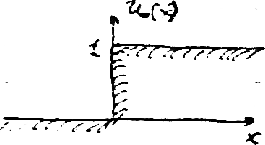
\includegraphics[width=0.2\textwidth]{9_1_new}
\end{center}
\item Увеличим ступеньку в $u_*$ раз и сдвинем.
$$u(t,x) = \frac{u_*}{2}\sbrs{1+\Phi \brs{\frac{x-x_0}{\sqrt{4a^2t}}}}$$
\item Можем получить и ступеньку конечной ширины.
$$u(t,x) = \frac{u_*}{2}\sbrs{\Phi \brs{\frac{x-x_1}{\sqrt{4a^2t}}}-\Phi \brs{\frac{x-x_2}{\sqrt{4a^2t}}}}$$
\item Для системы из $N$ интервалов имеем:
\begin{center}
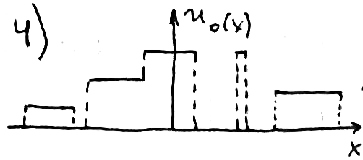
\includegraphics[width=0.2\textwidth]{9_2_new}
\end{center}
$$u(t,x) = \sum_{k=1}^{N}\frac{u_{*k}}{2}\sbrs{\Phi \brs{\frac{x-x_{1k}}{\sqrt{4a^2t}}}-\Phi \brs{\frac{x-x_{2k}}{\sqrt{4a^2t}}}}$$
Последнее можно переписать в следующем виде:
$$u(t,x) = \sum_{k=1}^{N}\sbrs{\frac{\fbrs{-\frac{1}{2}\Phi \brs{\frac{x-x_{2k}}{\sqrt{4a^2t}}}}-\fbrs{-\frac{1}{2}\Phi \brs{\frac{x-x_{1k}}{\sqrt{4a^2t}}}}}{x_{2k}-x_{1k}}}u_{*k} (x_{2k} - x_{1k})$$
\item Окончательно, пусть $u_0(x)$ финитна, непрерывна, ограничена. Разбиваем ее носитель $\mathrm{supp}\; u_0(x)$ на отрезки, аппроксимируем кусочно постоянной. Для приближенных решений справедливо:
\begin{align*}
u(t,x) &= \sbrs { \Psi (t,x, \xi) = -\frac{1}{2}\Phi \brs{\frac{x - \xi}{\sqrt{4a^2t}}}} = \sum \frac{\Psi(t,x,x_{2k})-\Psi(t,x,x_{1k})}{x_{2k}-x_{1k}} u_0 \brs{\frac{x_{2k}+x_{1k}}{2}} \brs{x_{2k}-x_{1k}} \approx\\
& \approx \sum_{k=1}^N \left. \pd{\Psi}{\xi}\right |_{\xi = \frac{x_{2k}+x_{1k}}{2}} u_0 \brs{\frac{x_{2k}+x_{1k}}{2}}\brs{x_{2k}-x_{1k}} = \sbrs{\pd{\Psi}{\xi} = \frac{1}{\sqrt{4 \pi a^2 t}} e^{-\dfrac{(x-\xi)^2}{4a^2t}}} = \\
&= \sum_{k=1}^N \frac{1}{\sqrt{4 \pi a^2 t}} \left. e^{-\dfrac{(x-\xi)^2}{4a^2t}} \right |_{\xi = \frac{x_{2k}+x_{1k}}{2}} u_{*k} \brs{x_{2k} - x_{1k}} - \text{ Интегральная сумма Римана}
\end{align*}
Предположение: решение будет $$u(t,x) = \frac{1}{\sqrt{4\pi a^2 t}} \int_{-\infty}^{\infty}e^{-\dfrac{(x-\xi)^2}{4a^2t}} u_0(y) dy - \text{ Формула Пуассона} $$
Функция $$\mathcal{E}(t,x) =  \frac{1}{\sqrt{4\pi a^2 t}} e^{-\dfrac{x^2}{4a^2 t}} - \textbf{фундаментальное решение (или функция источника)}$$
\end{enumerate}
\begin{theorem}
Пусть $u_0\in C(\bR^1),\ \abs{u_0(x)}\leq M_0\ \forall x\in \bR^1$. Тогда функция $u(t,x) = \dfrac{1}{\sqrt{4\pi a^2 t}} \displaystyle\int_{-\infty}^{\infty}e^{-\dfrac{(x - y)^2}{4a^2t}} u_0(y) dy$
\begin{enumerate}
\item Принадлежит классу $C^{\infty}(t>0, x\in\bR^1)\cap C(t\geq 0, x\in\bR^1)$
\item Является классическим решением задачи Коши
\begin{equation*}
\begin{cases}
	u_t - a^2u_{xx} = 0, t > 0, \; x \in \R^3, \\
	u\bigr|_{t = 0} = u_0(x), \; x \in \R
\end{cases}
\end{equation*}
\item $\abs{u(t,x)}\leq M\ \forall t \geq 0,x\in\bR^1$
\end{enumerate}
\end{theorem}
\begin{proof}
\begin{enumerate}
\item 
В исходном интеграле для $u(t,x)$ сделаем такую замену:
\[
\frac{y-x}{2a\sqrt{t}}=\eta ,\ y=x+2a\sqrt{t}\eta ,\ dy=2a\sqrt{t}d\eta
\]
Тогда получим
\[
u(t,x)=\frac{1}{\sqrt{\pi}}\int_{-\infty}^{\infty}e^{-\eta^2} u_0(x+2a\sqrt{t}\eta) d\eta,\ u_0(x+2a\sqrt{t}\eta)  \in C(t\geq 0, x\in\bR^1,\eta\in\bR^1)
\]
Оценим $\abs{e^{-\eta^2} u_0(x+2a\sqrt{t}\eta)}\leq M_0e^{-\eta^2}$, причем $\displaystyle\int_{-\infty}^{\infty}M_0e^{-\eta^2}d\eta <\infty\Rightarrow$ этот интеграл сходится абсолютно и равномерно, а значит лежит в $C(t\geq 0, x\in\bR^1)$. Отсюда следует третье утверждение теоремы.

Возьмем 
\[
u_x(t, x)\sim \int_{-\infty}^{\infty}\frac{1}{4a^3\sqrt{\pi}t^{3/2}}e^{-\dfrac{(x-y)^2}{4a^2t}} (y-x)u_0(y) dy=J, 
\]
где выражение под интегралом лежит в $C(t\geq 0, x\in\bR^1,\eta\in\bR^1)$.
Покажем равномерную сходимость этого интеграла серией оценок:

\begin{enumerate}
\item $\abs{y-x}\geq \abs{y}-A,\ \abs{x}<A,\ y\in\bR$
\item $\abs{y-x}\leq \abs{y}+A$
\item При $\abs{y}>A$ : $(y-x)^2\geq (\abs{y}-A)^2=y^2+A^2-2\dfrac{\abs{y}}{\sqrt{2}}(\sqrt{2}A)\geq y^2+A^2-\dfrac{y^2}{2}-2A^2=\dfrac{y^2}{2}-A^2$.

При $\abs{y}\leq A\ : (x-y)^2>-\dfrac{A^2}{2}$.
\item Возьмем
\[
\phi_A(y)=\begin{cases}
-\dfrac{y^2}{2}-A^2,\ &\abs{y}\geq A\\
-\dfrac{A^2}{2},\ &\abs{y}<A
\end{cases}
\]
Тогда $(x-y)^2\geq\phi_A(y)\ \forall x\leq A,y\in\bR$.
\end{enumerate}
Получили следующую оценку:
\[
\abs{\frac{1}{4a^3\sqrt{\pi}t^{3/2}}e^{-\dfrac{(x-y)^2}{4a^2t}} (y-x)u_0(y)}\leq \frac{M_0}{4a^3\sqrt{\pi}t^{3/2}}(\abs{y}+A)e^{-\dfrac{\phi_A(y)}{4a^2t}}
\]
Этот интеграл сходится при ограничения на $t$, т.е. в прямоугольнике $Q=\{t\in (t_1, t_2),x\in (-A, A)\}$, т.е. есть равномерная сходимость $J$ в любом прямоугольнике. Беря в качестве $Q$ всевозможные такие прямоугольники, получим $J\in C(t\geq 0, x\in\bR^1)$. Аналогично будет для любой другой производной (будет асимптотика $\abs{P_n(y)}e^{-\alpha y^2}$).
\item $\ $
\[
\begin{split}
&\mathcal{E} (t, x-y)=\frac{1}{\sqrt{4\pi a^2t}}e^{-\frac{(x-y)^2}{4a^2t}}\\[7pt] 
&\mathcal{E}_x (t, x-y)=-\frac{(x-y)}{{2\sqrt{\pi} 2a^3t^{3/2}}}e^{-\frac{(x-y)^2}{4a^2t}}\\[7pt]
&\mathcal{E}_{xx} (t, x-y)=\frac{1}{2\sqrt{\pi}}\left[\frac{-1}{2a^3t^{3/2}}+\frac{(x-y)^2}{4a^5t^{5/2}} \right]e^{-\frac{(x-y)^2}{4a^2t}}\\[7pt] 
&\mathcal{E}_t (t, x-y)=\frac{1}{2\sqrt{\pi}}\left[\frac{-1}{2at^{3/2}}+\frac{(x-y)^2}{4a^3t^{5/2}} \right]e^{-\frac{(x-y)^2}{4a^2t}}
\end{split}
\]
Тогда 
\[
u_t-a^2u_{xx}=\int\limits_{-\infty}^{+\infty}\cancelto{0}{\left[\mathcal{E}_t(t, x-y)-a^2\mathcal{E}_{xx}(t, x-y) \right]}u_0(y)dy=0.
\]
Начальное условие (используя самое начало выкладок)
\[
\while{u}{t=0}=\frac{1}{\sqrt{\pi}}\int\limits_{-\infty}^{+\infty}e^{-\eta^2}u_0(x)d\eta = u_0(x)
\]
\end{enumerate}
Теорема доказана.
\end{proof}




